%%% 特別研究報告書サンプル
\documentclass[dvipdfmx]{ampbt_nomag}

%%% クラスオプション:
%%% chapter: \chapterコマンドを使用可能にする(jsbook (report) を使う).
%%% その他 jsclasses に指定可能なオプションが指定できます(そのまま渡される).

%%% 題目 %%%%%%%%%%%%%%%%%%%%%%%%%%%%%%%%%%%%%%%%%%%%%%%%%%%%%%%%%%%%%%%%%%%%%%%%
\title{方策学習による低次元行動空間抽出と
}     % 題目1行目
      {実環境における物体操り動作獲得}                             % 題目2行目
      {}                                              % 題目3行目
%%% 指導教員 %%%%%%%%%%%%%%%%%%%%%%%%%%%%%%%%%%%%%%%%%%%%%%%%%%%%%%%%%%%%%%%%%%%%
\supervisors{森本淳}{教授}    % 指導教員1人目 {氏名}{職名}
            {}{}    % 指導教員2人目 {氏名}{職名}
            {}{}                % 指導教員3人目 {氏名}{職名}
%%% 入学年月 %%%%%%%%%%%%%%%%%%%%%%%%%%%%%%%%%%%%%%%%%%%%%%%%%%%%%%%%%%%%%%%%%%%%
\entrancedate{2022}{4}          % {年}{月}
%%% 著者氏名 %%%%%%%%%%%%%%%%%%%%%%%%%%%%%%%%%%%%%%%%%%%%%%%%%%%%%%%%%%%%%%%%%%%%
\author{古巻}{鉄平}             % {姓}{名}
%%% 提出日 %%%%%%%%%%%%%%%%%%%%%%%%%%%%%%%%%%%%%%%%%%%%%%%%%%%%%%%%%%%%%%%%%%%%%%
\submissiondate{2024}{2}{5}    % {年}{月}{日}
%%% 背表紙の幅 %%%%%%%%%%%%%%%%%%%%%%%%%%%%%%%%%%%%%%%%%%%%%%%%%%%%%%%%%%%%%%%%%%
\setlength{\wdspine}{15mm}
%%% 背表紙の出力枚数 %%%%%%%%%%%%%%%%%%%%%%%%%%%%%%%%%%%%%%%%%%%%%%%%%%%%%%%%%%%%
\def\numberofspines{1}
%%% 摘要 %%%%%%%%%%%%%%%%%%%%%%%%%%%%%%%%%%%%%%%%%%%%%%%%%%%%%%%%%%%%%%%%%%%%%%%%
\abstract{%
}
%%% パッケージの読み込みや自分用のマクロの定義 %%%%%%%%%%%%%%%%%%%%%%%%%%%%%%%%%%
\usepackage{amsmath,amssymb}
\usepackage{algorithmic}
\usepackage{algorithm}
\usepackage{graphicx}
\usepackage{dsfont}

\usepackage[subrefformat=parens]{subcaption}


%%%\usepackage{bxpapersize} %%%消すべき?
\newcommand{\rme}{\mathrm{e}}
\renewcommand{\bfdefault}{bx}


%%% 出力の制御 %%%%%%%%%%%%%%%%%%%%%%%%%%%%%%%%%%%%%%%%%%%%%%%%%%%%%%%%%%%%%%%%%%

%%% 本文を出力しない場合,次の行のコメントを外して下さい.
%%\outputbodyfalse

%%% 末尾に表紙,背表紙を出力しない場合,次の行のコメントを外して下さい.
%% \outputcoverfalse

%%% 末尾に提出用摘要を出力しない場合,次の行のコメントを外して下さい.
%% \outputabstractforsubmissionfalse

%%% ampbt.cls では表紙等の作成のために geometry パッケージを使用しているため,本文
%%% のレイアウトを変えるために \usepackage[...]{geometry} とすると Option clash が
%%% 発生します.何らかの理由で本文のレイアウトを変更したい場合は \geometry{...} を
%%% 使用して下さい.
%%% また,jsclasses を使用しているため,例えば 3cm を指定したい場合は 3truecm と書
%%% く必要があります.
%% \geometry{hmargin=3truecm,vmargin=2truecm}

\begin{document}
\ifoutputbody
%%% 中表紙,摘要,目次 %%%%%%%%%%%%%%%%%%%%%%%%%%%%%%%%%%%%%%%%%%%%%%%%%%%%%%%%%%
\makeinsidecover                % 中表紙
\makeabstract                   % 摘要
\maketoc                        % 目次
\setcounter{page}{1}            % 本文のページ番号を1から始める
%%% 本文 %%%%%%%%%%%%%%%%%%%%%%%%%%%%%%%%%%%%%%%%%%%%%%%%%%%%%%%%%%%%%%%%%%%%%%%%
\section{序論}\label{sec-intro}		% 本文の開始
人間の手を模倣した多指ハンドロボットの実用化は社会的に大きな意義がある.人間が日常生活を送るにあたって手で物体を操るという動作は必要不可欠であるが,多指ハンドロボットが実現することでこれらの動作を代替することができる.このような多指ハンドロボットには,多種多様な形状を持つ物体を操る能力が要求される.これまで様々な多指ハンドロボットの開発が進められてきたものの,多指ハンドロボットを人間のように器用に動かす制御手法については依然として開発が進んでおらず実用化とは程遠い状況にある.\\
%%% 「このような多指ハンドロボットには,多種多様な形状を持つ物体を操る能力が要求される.」という文章はどこかには絶対欲しいが場所を間違えている気がする.
多指ハンドロボットの制御手法の開発では,操作する物体との間に接触が多くモデル化が困難である点が特に問題となる.このような課題を解決するため,多指ハンドロボットの制御手法としてモデルフリー強化学習がよく用いられる.モデルフリー強化学習では力学モデルの存在を陽に仮定せず,環境との相互作用を繰り返すことによって制御方策を獲得する\cite{RLBook}.一方で,モデルフリー強化学習は複雑なタスクの学習を可能にしたものの,あるタスクを学習して得られた方策を環境のわずかに異なる別のタスクに適用するのは困難である\cite{hua2021learning}.このため,多指ハンドロボットの目的である様々な形状の物体の操作を達成することが出来ない.\\
%%% 「環境」「タスク」という用語を突然登場させないほうが良い?
このようなモデルフリー強化学習の課題を解決するために(12月8日ミーティングでの話を考慮して書く.「階層強化学習」ではない.「オプション」「downstream task」あたりの話をまとめて書く.)
\\
本研究ではこのような〜〜〜を用いて複数の形状のバルブを短時間で学習させる.\\
(実験結果)\\

\clearpage
\section{関連研究}\label{sec-related_papers}
%%% オプションやdownstreamの話を入れ込む形で修正する.

\subsection{多指ハンドロボットのハードウェア}
・多指ハンドロボットは古くから開発されてきた.\\
  ・ワイヤ駆動のロボット:Shadow Adroit\cite{kumar2014real}\\
  ・Direct-drivenなどロボット:Allegro\\
・しかし,これらのロボットは費用が高く,故障時の修理が困難である.\\
%%% もう一種類挙げたい.
・近年は低価格かつ修理が容易なトイロボットであるRobel\cite{ahn2020robel},LEAP hand\cite{shaw2023leap}などが強化学習の研究に用いられている.\\
%%% LEAP handは最近出たばかりなので強化学習の研究によく用いられるではおかしい.
%%% 接触センサの話は不要?博士の研究を視野に入れるなら...?

\subsection{多指ハンドロボットの低次元制御}
・多指ハンドロボットは次元が多い.
・義手の分野で多指ハンドロボットの次元を下げられる.
・PCAを用いることで
・VAEなど非線形のマッピングを用いることでより高精度な次元圧縮が可能.


\subsection{接触の多いタスクの制御}
・強化学習を用いている研究をいくつか\\
・目的は,現状どこまで出来ているかを明らかにすること.\\
・OpenAIのルービックキューブの研究など.\\

\subsection{事前データを用いた強化学習}
事前に収集したデータから複数のタスクの学習を効率化するための手段として,スキルの事前学習が研究されている.スキルの事前学習では,情報が付加されていないデータを収集し,そのデータからスキルを抽出する.その後,抽出したスキルを行動として利用することで学習する.Singhらは,正規化フロー法\cite{dinh2016density}を用いて標準正規分布に従うノイズベクトルを行動ベクトルへ射影することで,学習速度を向上させる行動の事前分布を獲得した\cite{singh2020parrot}.また,Pertschらは,事前に収集したデータから行動の系列をサンプリングし,変分オートエンコーダ(VAE)によってサンプリングした系列の再構成学習を行うことで,スキルを潜在空間上に埋め込み高速な学習を実現する手法を開発した\cite{pertsch2021accelerating}.本研究では事前に収集したデータからスキルを抽出することでハンドロボットの回転タスクについて,未知のタスクに対する学習速度を向上させる手法を検討する.

\clearpage
\section{手法}\label{sec-method}
\subsection{強化学習(整理し直す)}
本研究ではロボットの制御問題をマルコフ決定過程$\mathcal{M} = (\mathcal{S},\mathcal{A},p,r)$によってモデリングする.$\mathcal{S}$,$\mathcal{A}$はそれぞれ状態空間,行動空間を意味しており,現在の状態$s_t \in \mathcal{S}$で行動$a_t \in \mathcal{A}$をとった時に状態$s_{t+1}\in\mathcal{S}$へと遷移する状態遷移確率を$ p:\mathcal{S}\times\mathcal{A}\times\mathcal{S}\rightarrow[0,1]$,この時エージェントが得る報酬を $r:\mathcal{S}\times\mathcal{A}\rightarrow\mathbb{R}$と表す.また,方策$\pi(a_t|s_t)$に従って行動した際に得られる状態と行動の系列において,$s_t$が表れる確率を$\rho_\pi(s_t)$,$s_t$と$a_t$が同時に表れる確率を$\rho_\pi(s_t,a_t)$,デモンストレーションデータの中に$s_t$と$a_t$が同時に現れる確率を$\rho_D(s_t,a_t)$ と表記する.\\
通常の強化学習では,累積報酬$\sum_t \mathbb{E}_{(s_t,a_t)\sim\rho_\pi}[r(s_t, a_t)]$を最大化することを目指す.ただし,実際はステップ数が無限大の時に発散しないために割引率$\gamma$の冪乗を$r$の前にかけることが多い.累積報酬の最大化に向け,まず各状態における状態価値関数と行動を含めた行動価値関数を以下のように定義する.
\begin{eqnarray} \label{state_value1}
  V_\pi(s) &=& \mathbb{E}_{\rho_\pi} \left[\sum^{\infty}_{k=0}\gamma^kr(s_{t+k},a_{t+k}) \middle|s_t = s\right] \\
  \label{state_value2}
  Q_\pi(s,a) &=& \mathbb{E}_{\rho_\pi} \left[\sum^{\infty}_{k=0}\gamma^kr(s_{t+k},a_{t+k}) \middle|s_t = s, a_t = a \right]
\end{eqnarray}
この時,式(\ref{state_value1})を
\begin{eqnarray} \label{bellman_equation}
  V_\pi(s) &=& \mathbb{E}_{\rho_\pi} \left[ r(s_t,a_t) + \sum^{\infty}_{k=1} \gamma^{k}r(s_{t+k},a_{t+k}) \middle|s_t = s\right] \\ \nonumber
  &=& \mathbb{E}_{\rho_\pi} \left[ r(s_t,a_t) + \gamma V_\pi(s_{t+1}) \middle|s_t = s\right]
\end{eqnarray}
のように変形することでベルマン方程式が得られる.式(\ref{bellman_equation})における期待値をとる操作を最大値をとる操作に置き換えたものをベルマン最適方程式と呼び,期待値をとるものはベルマン期待方程式と呼ぶ.このベルマン方程式の右辺を$V_\pi(\cdot)$の写像と見做すことで次のようなベルマン作用素$\mathcal{T}^\pi$を定義する.
\begin{eqnarray} \label{bellman_operator}
  \mathcal{T}^\pi\circ V(s) &=&  \mathbb{E}_{\rho_\pi} \left[ r(s_t,a_t) + \gamma V(s_{t+1}) \middle|s_t = s\right]
\end{eqnarray}
式(\ref{state_value2})の状態価値関数についても同様にベルマン方程式やベルマン作用素を定義できる.特に,ベルマン期待方程式についての作用素をベルマン期待作用素,ベルマン最適方程式についての作用素をベルマン最適作用素と呼ぶ.ベルマン作用素は縮小写像であるため$V_\pi(s)$はランダムな初期値から何度もベルマン作用素を作用させることにより真の関数に収束する.\\
このような価値関数を求めるための方法は,動的計画法,モンテカルロ法,TD法の3種類に大別される.動的計画法は環境の情報が既知であると仮定した上でベルマン方程式を解く手法で,ベルマン期待作用素による方策の評価と改善を繰り返す方策反復とベルマン最適作用素を用いて最適な方策を求める価値反復に大別できる.
モンテカルロ法はエージェントが探索して得られた経験をもとに学習する.エージェントが探索した1エピソード分の系列を用いて方策や価値関数を更新する.
TD法は,動的計画法においてある状態の価値関数を推定する際に一つ前の状態の推定値を利用するという特性と,モンテカルロ法におけるエージェントの経験を利用するという特性を組み合わせたもので,1ステップごとに更新する.TD法を使ったアルゴリズムとして方策オン型のSARSAや方策オフ型のQ-leraningが存在する.\\
通常の強化学習は状態空間,行動空間が離散の場合,価値関数を表形式で保存することにより実行できるが,状態空間と行動空間が大きい場合や連続な場合,価値関数を表形式で表すと膨大なメモリを必要とする.ロボット制御では連続な物理系を考えるため価値関数は表形式ではなく近似器のパラメータとして保存し,最適化したい目的関数に応じて更新する.

\subsection{エントロピー最大強化学習}


\subsection{Soft Actor-Critic法(分割する)}
Soft Actor-Critic(SAC)\cite{SAC1,SAC2}は連続な行動空間上で学習できる方策オフ型強化学習アルゴリズムである.このようなActor-criticアルゴリズムは方策を保存するActorと価値関数を保存するCriticという二つのネットワークを持っておりこれらを更新することによって学習する.\\
状態価値関数は累積報酬に探索を促進するためのエントロピー項を加えた式(\ref{sac_state_value})で表される.この時,実際は報酬に割引率がかけられており,また,エントロピーの項に存在する$\alpha$は温度パラメータである.温度パラメータは学習が進むにつれて小さくしてゆくことで最終的な方策を決定的な方策に近づける.
\begin{equation} \label{sac_state_value}
 V(s_t) = \mathbb{E}_{a_t\sim\pi}\left[r(s_{t},a_{t}) - \alpha \textrm{log}\pi (a_{t}|s_{t}) \right] 
\end{equation}
また,行動価値関数は先ほどの状態価値関数を用いて,
\begin{equation} \label{sac_act_value}
  Q(s_t,a_t) = r(s_{t},a_{t})+\gamma \mathbb{E}_{a_t\sim p}[V(s_{t+1})]
\end{equation}
のように表すことができる.これを式(\ref{sac_state_value})に代入することで
\begin{equation} \label{sac_v_q}
  V(s) = \mathbb{E}_{a_t\sim\pi} \left[Q(s,a) - \alpha \textrm{log}~\pi (a|s)  \right]
\end{equation}
という式が得られる.一方,SACにおいて方策はガウス方策であるものとし,平均と分散によってパラメータ化する.このような方策を価値関数を最大にするよう以下のように更新を行う.なお,$\Pi$はガウス方策全体からなる集合を意味する.
\begin{equation} \label{sac_policy_iter}
  \pi_{\mathrm{new}} = \mathop{\textrm{argmin}}_{\pi'\in\Pi}D_\mathrm{KL}\left(\pi'(\cdot|s_t) \bigg\Vert
  \frac{\exp(Q^{\pi_{old}}(s_t,\cdot))}{Z^{\pi_{old}}(s_t)} \right).
\end{equation}
次にこれらの価値関数や方策を関数近似器で表現する.soft-Q関数は$Q_\theta(s_t,a_t)$,方策は$\pi_\phi$のように表記する.今回の実験では関数近似器としてニューラルネットワークを用いるため,$\theta,\phi$はネットワークのパラメータを表す.\\
soft-Q関数の損失関数を
\begin{align} \label{sac_value_loss}
  J_Q(\theta) &= \mathbb{E}_{(s_t,a_t) \sim D} \left[ \frac{1}{2}\left( Q_\theta(s_t,a_t) - \bar{Q}_{\bar{\theta}}(s,a) \right)^2 \right], \\
  \bar{Q}_{\bar{\theta}} &= r(s_t,a_t) + \gamma \mathbb{E}_{s_{t+1} \sim p}[V_{\bar{\theta}}(s_{t+1})],
\end{align}
のように表す.
ただし,$V_{\bar{\theta}}(s_{t+1})$はsoft-Q関数から$Q=\bar{Q}_{\bar{\theta}}$として式(\ref{sac_v_q})を使って求める.
また,$\bar{\theta}$はtarget-Q関数$\bar{Q}_{\bar{\theta}}$のパラメータで,soft-Q関数のパラメータの指数加重移動平均として計算される.
式(\ref{sac_value_loss})の勾配は1ステップのサンプルで期待値を近似することで,
\begin{eqnarray}
  \hat{\nabla}J_Q(\theta) = \nabla_\theta Q_\theta\biggl(Q_\theta - \Bigl(r(s_t,a_t) + \gamma \bigl(Q_\theta - \alpha \textrm{log}(\pi_{\phi}(a_{t+1}|s_{t+1}))\bigl)\Bigl)\biggl),
\end{eqnarray}
のようになる.
soft-Q関数を実装する際は,SACでは方策改善における正のバイアスを軽減するため2つのQ関数を同時に学習させ,ある状態行動対を評価する際にはこれらのうち値の小さい方を利用する\cite{DoubleQ}.
そのため,target-Q関数も合わせて合計で4つのネットワークで学習することとなる.
方策の損失関数は式(\ref{sac_policy_iter})のKLダイバージェンスを最小にするため以下のように計算する.
\begin{equation} \label{sac_policy_loss}
  J_\pi(\phi) = \mathbb{E}_{s_t \sim D,a_t\sim\pi_\phi(\cdot|s_t)} \left[\textrm{log}\pi_\phi(a_t | s_t) - Q_\theta(s_t,a_t)\right].
\end{equation}
この損失関数は行動$a_t$についての期待値を取っているが,$a_t$は$\pi_\phi(\cdot|s_t)$からサンプリングしたものなので先ほどのように勾配を求めることはできない.$\pi_\phi(\cdot|s_t)$はガウス分布であることから,ニューラルネットワークでガウス分布の平均と標準偏差を求めそれを基に$a_t$を構成するreparameterized trickによって勾配を求める.この時,$a_t$は標準正規分布からサンプリングした$\varepsilon_t$を用いて
\begin{equation} \label{reparameterization}
  a_t = f_\phi(\varepsilon_t;s_t),
\end{equation}
と表すと,式(\ref{sac_policy_loss})は
\begin{equation} \label{sac_policy_loss_reparameterized}
  J_\pi(\phi) = \mathbb{E}_{s_t \sim D,\varepsilon_t \sim \mathcal{N}(0,1)} \left[\textrm{log}\pi_\phi(f_\phi(\varepsilon_t;s_t) | s_t) - Q_\theta(s_t,f_\phi(\varepsilon_t;s_t))\right],
\end{equation}
のように変形でき,この勾配は
\begin{equation} \label{sac_policy_gradient}
  \hat{\nabla}_\phi J_\pi(\phi) = \nabla_\phi \alpha \textrm{log}\pi_\phi(a_t|s_t) + \nabla_\phi f_\phi(\varepsilon_t;s_t)[\nabla_{a_t}\alpha \textrm{log} \pi_\phi(a_t|s_t) - \nabla_{a_t}Q_\theta(s_t,a_t)],
\end{equation}
として計算できる.
また,エントロピー項にかかっている温度パラメータは以下のような目的関数の勾配を取ることによって更新をおこなう\cite{SAC2}.
この時,$\bar{\mathcal{H}}$は目標エントロピーを表している.
\begin{equation} \label{temparature_tunning}
  J(\alpha) = \mathbb{E}_{a_t\sim\pi_t}[-\alpha \log{\pi_t(a_t|s_t)} -\alpha\bar{\mathcal{H}}].
\end{equation}

\subsection{変分自己符号化器}

%%% 基本的な説明と潜在変数モデル
% VAEがニューラルネットワークを用いた生成モデルである.
% 教師なし学習
% 潜在変数モデル
変分自己符号化器(VAE)は,ニューラルネットワークを用いた代表的な生成モデルのアルゴリズムであり,画像処理などの分野で利用されてきた.VAEはその名の通り自己符号化器と類似した構造を持つ教師なし学習アルゴリズムである.VAEは訓練データを潜在変数として抽象化し,抽象化した潜在変数からもとの訓練データに復元することを学習し,これによって訓練データ全体の確率分布とそれらの抽象的な特徴表現を獲得する.\\
%%% VAEの学習メカニズム
% 生成モデルにおける目的関数
VAEはあるデータセット$\mathcal{D}=\{\boldsymbol{x}_i\}^{N}_{i=1}$を生成するような確率分布$p(\boldsymbol{x})$を近似する生成モデル$p_\theta(\boldsymbol{x})$の獲得を目指す.このような確率分布を学習するにあたって,$\boldsymbol{x}$がある潜在変数$\boldsymbol{z}\sim p(\boldsymbol{z})$に従って生成されると仮定する.このとき,事後確率分布$p(\boldsymbol{z}|\boldsymbol{x})$をパラメータ$\phi$を用いて$q_\phi(\boldsymbol{z}|\boldsymbol{x})$のように近似することを考えると,生成モデルは以下のように変形できる.

\begin{equation} \label{latent_val}
  \log{p_\theta(\boldsymbol{x})} = D_{KL}(q_\phi(\boldsymbol{z}|\boldsymbol{x})||p_\theta(\boldsymbol{z}|\boldsymbol{x})) + \mathcal{L}(\theta, \phi; \boldsymbol{x})
\end{equation}

右辺の第1項は0以上であることから,$\log{p_\theta(\boldsymbol{x})} \geq \mathcal{L}(\theta, \phi; \boldsymbol{x})$が成り立つため,$p_\theta(\boldsymbol{x})$の代わりに
\begin{equation} \label{ELBO}
  \mathcal{L}(\theta, \phi; \boldsymbol{x}) = \mathbb{E}_{q_\phi(\boldsymbol{z}|\boldsymbol{x})}[\log{p_\theta(\boldsymbol{x}|\boldsymbol{z})}]-D_{KL}(q_\phi(\boldsymbol{z}|\boldsymbol{x})||p_\theta(\boldsymbol{z}))
\end{equation}
を最大化することで生成モデルを獲得できる.このような$\mathcal{L}(\theta, \phi; \boldsymbol{x})$のことをエビデンス下界(ELBO)と呼ぶ.\\
% エンコーダとデコーダ
パラメータ表示された尤度$p_\theta(\boldsymbol{x}|\boldsymbol{z})$と近似事後確率分布$q_\phi(\boldsymbol{z}|\boldsymbol{x})$はニューラルネットワークで表現される.尤度$p_\theta(\boldsymbol{x}|\boldsymbol{z})$は潜在変数$\boldsymbol{z}$を入力すると再構成された$\boldsymbol{x}$を出力するネットワークでありデコーダと呼ばれる.また,近似事後確率分布は$\boldsymbol{x}$を入力すると,潜在変数$\boldsymbol{z}$の平均$\mu_{\boldsymbol{z}}(\boldsymbol{x})$と分散の対数$\log{\sigma_{\boldsymbol{z}}^2(\boldsymbol{x})}$を出力するネットワークで,エンコーダと呼ばれる.潜在変数$\boldsymbol{z}$は標準正規分布$\mathcal{N}(0,\boldsymbol{I})$に従う確率変数であり,エンコーダでは標準正規分布に従う変数$\boldsymbol{\varepsilon} \sim \mathcal{N}(0,\boldsymbol{I})$を用いて
\begin{equation} \label{VAE_latent_val}
\boldsymbol{z} = \mu_{\boldsymbol{z}}(\boldsymbol{x}) + \sigma_{\boldsymbol{z}}(\boldsymbol{x}) * \boldsymbol{\varepsilon}
\end{equation}
のように計算する.\\
% 損失関数
このとき,ELBOの第1項は
\begin{equation} \label{ELBO_RHS_1}
  \mathbb{E}_{q_\phi(\boldsymbol{z}|\boldsymbol{x})}[\log{p_\theta(\boldsymbol{x}|\boldsymbol{z})}] = \mathbb{E}_{\boldsymbol{\varepsilon} \sim \mathcal{N}(0,\boldsymbol{I})} [\log{p(x|\mu_{\boldsymbol{z}}(\boldsymbol{x}) + \sigma_{\boldsymbol{z}}(\boldsymbol{x}) * \boldsymbol{\varepsilon})}]
\end{equation}
のようにサンプリングを用いて計算され,第2項は
\begin{equation} \label{ELBO_RHS_2}
  D_{KL}(q_\phi(\boldsymbol{z}|\boldsymbol{x})||p_\theta(\boldsymbol{z})) = -1/2 \sum^N_{i=1}\log{{\sigma_{\boldsymbol{z}}^2(\boldsymbol{x_i})}} - 1 + \mu_{\boldsymbol{z}}^2(\boldsymbol{x_i}) + \sigma_{\boldsymbol{z}}^2(\boldsymbol{x_i})
\end{equation}
のように解析的に計算できる.

%%% VAEと研究の関連性
% VAEが義手や多指ハンドロボットの研究においてどのように応用されるか
% 今回の研究においてVAEはどのように利用されるか.
VAEを用いることで非線形な次元圧縮を行うことができ,義手をはじめとする多指ハンドロボットの研究において,VAEは多次元の制御入力を低次元に圧縮するため利用される\ref{}\ref{}.本研究ではVAEの学習によって獲得した低次元の潜在空間を強化学習における行動空間として利用することで効率的な強化学習を実現する.




\subsection{低次元行動空間の抽出}

行動空間が高次元であるタスクの学習にあたって,事前データを用いてその学習を効率化させるアプローチが一般的である.Pertschらが提案したSPiRLは事前に収集したデータを基に,行動の系列を時間的・空間的に圧縮することで低次元の行動空間を獲得する.さらに各状態において低次元行動空間のどの行動が選択されるかについての事前分布も同時に学習することで強化学習を高速化する\cite{pertsch2021accelerating}.本研究ではSPiRLをベースとしたアルゴリズムを利用する.\\
SPiRLの学習に用いるデータセット$\mathcal{D}=\{\tau_i\}^{N}_{i=1}$はN個の系列から構成されており,各系列は$\tau_i = {(s_0, a_0), . . . ,(s_T, a_T)}$といったように$T$個の状態行動対で構成される.低次元行動空間の抽出には,これらのデータセットから連続したH個の行動をサンプリングし,その行動列$\boldsymbol{a}=\{a_l,a_{l+1},a_{l+H}\}$について,前節のようにELBOを最大化することで学習する.このとき,式(\ref{ELBO})における右辺第2項のKLダイバージェンスには以下のように再構成項と正規化項を調整するために$\beta$という係数がかけられている.
\begin{eqnarray} 
  \label{SPiRL_ELBO}
  \log p(\boldsymbol{a}) &\geq& \mathbb{E}_q [\log p(\boldsymbol{a}|z)  -\beta(\log{q(z|\boldsymbol{a})} - \log{p(z)})]
  \end{eqnarray}

% SPiRLでは系列を集めたデータセットを用いる.
% SPiRLの学習は1)スキルからの低次元行動空間の抽出,2)事前分布の
% 本研究ではSPiRLと同様に低次元行動空間の抽出によって,


また,低次元行動空間の獲得と同時に,低次元行動空間上の学習を促進するための事前分布$p_{\boldsymbol{a}}(z|s_t)$も学習し,各状態$s_t$において実行すべき低次元の行動に関する情報を抽出する.このような事前分布は以下のようなKullback--Leiblerダイバージェンスが最小になるよう学習する.
\begin{equation}
  \mathbb{E}_{(s,\boldsymbol{a}_i)\sim D}D_\mathrm{KL}\left(q(z|\boldsymbol{a}_i)\|p_{\boldsymbol{a}}(z|s_t)\right)
\end{equation}
低次元行動空間の獲得と事前分布の学習後,低次元行動空間上で強化学習を実行することでタスク達成可能な.この手法において方策は行動$a_t$の代わりにスキルの潜在変数$z$を出力する.出力された潜在変数$z$を学習したデコーダーに入力し,そこから出力された行動の系列を環境に入力する.このような方策$\pi_\theta(z|s_t)$のパラメータのを通常の強化学習の枠組みを用いて更新する.\\
本研究ではSPiRLにおける低次元行動空間の抽出とその空間上での強化学習について,実機環境における接触の多いマニピュレーションタスクに適用する.

\subsection{提案するフレームワーク}
本研究では,シミュレーション環境における低次元行動空間に抽出が,データセットとは異なるシミュレーション環境や実機における強化学習が高速化することを示す.研究手法は1)事前方策を用いたデータセットの収集2)低次元行動空間の抽出3)低次元行動空間上での強化学習という3つの要素から構築される.
事前方策を用いたデータセットの収集では,まず,シミュレーション環境上で事前方策を学習する.学習を繰り返したのち,目的となるタスクを達成可能な方策から系列データを生成し,それをデータセットに加える.その後行う低次元行動空間を抽出は,先ほど生成した軌道のデータセットを基にVAEを学習することによって行う.その後,獲得した低次元行動空間を用いて強化学習を実行する.この時,強化学習を実行する環境は使用する多指ハンドロボットが同じであれば操る物体はデータセットの収集時に使用しなかった物体でもよく,またロボットはシミュレーション上でも実機でもどちらでも同じように学習できる.\\
以上3つ要素を組み合わせたものが本研究で検証するフレームワークであり,その概要を図\ref{schematic_figure}に示した.次項では,本フレームワークの有効性を多指ハンドロボットにおけるバルブ回転タスクを用いて示す.

\begin{figure}[hbtp]
  \centering
  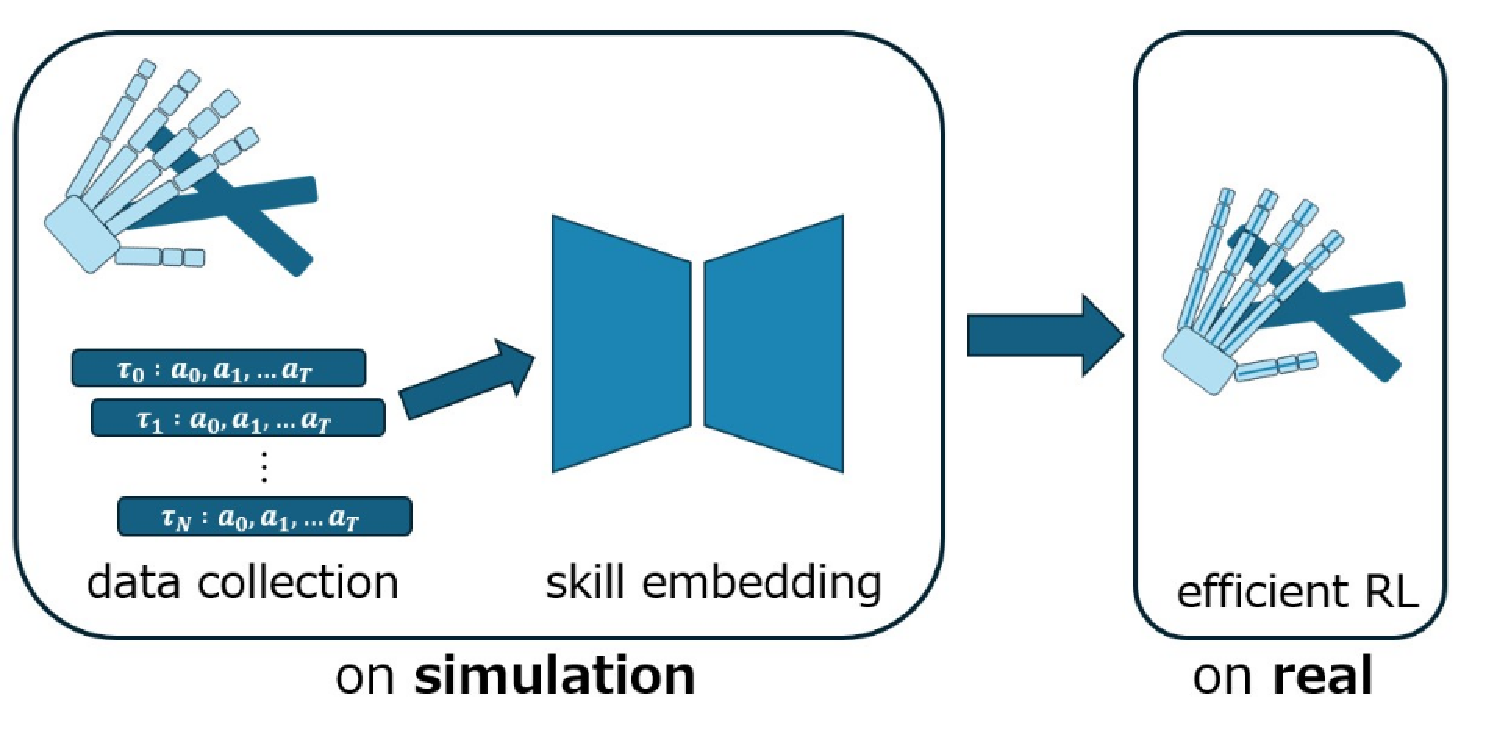
\includegraphics[width=17cm]
       {asset/img/schematic_figure.pdf}
  \caption{提案手法の概要}
  \label{schematic_figure}
\end{figure}

\clearpage
\section{実験}\label{sec-experiment}
前項で提案したフレームワークの性能を3指ハンドロボットのシミュレーション,および実機実験を通じて検証する.シミュレーション,実機ともに複数種類のバルブについて学習を行い,様々な形状のバルブにおいてこのフレームワークが有効であることを示す.

\subsection{実験のセットアップ}
本項では実験で利用する3指ハンドロボットD'Clawの構造とタスクの設定,シミュレーション環境と実機の設定について述べる.

\subsubsection{3指ハンドロボット:D'Claw}
\begin{figure}[hbtp]
  \centering
  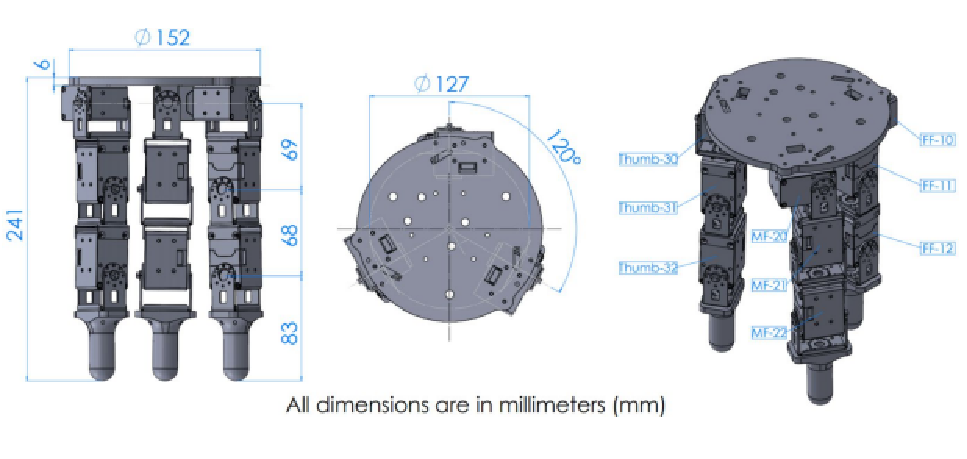
\includegraphics[height=6cm]
       {asset/img/dclaw.pdf}
  \caption{D'Clawの概要.FF-10$\sim$Thumb-32までの角度を$\theta^1_{\textrm{j}}\sim\theta^9_{\textrm{j}}$とし,$\boldsymbol{\theta}_{\textrm{j}}=(\theta^1_{\textrm{j}},\cdots,\theta^9_{\textrm{j}})$とおく.また,バルブの角度を$\theta^{\textrm{v}}$のように表記する.\cite{ahn2020robel}より引用.}
  \label{dclaw_structure}
\end{figure}
 
本研究ではオープンソースロボットプラットフォームRobelのハンドロボットD'Clawで実験する\cite{ahn2020robel}.D'Clawの構造は図\ref{dclaw_structure}に示している.D'Clawは3本の指を持ち,各指にはそれぞれ3つずつの関節,合わせて9つの関節が存在する.3本の指が持つ3つ関節の可動域はそれぞれ異なる.全関節が鉛直方向に垂れ下がった姿勢を中心とし前後に同角度の可動域を持ち,根本から$27.5^\circ,60^\circ,90^\circ$ずつ動かすことができる.\\
%%% (-27.5~27.5)であることが伝わっていなさそう.\\
ロボットの行動空間はロボットの関節の数と同じ9次元であり,各関節の目標角度を可動域の大きさで$[-1,1]$の範囲にスケールしたものを入力とする制御周期0.1sの位置制御である.状態空間は以下のように関節の角度$\boldsymbol{\theta}^{\textrm{j}}$,1ステップ前に実行した行動$\dot{\boldsymbol{\theta^{\textrm{j}}}}$,バルブの角度の余弦$\textrm{cos}(\theta^{\textrm{v}})$,バルブの角度の正弦$\textrm{sin}(\theta^{\textrm{v}})$,バルブの角度と目標角度の誤差$\theta^{\textrm{v}} - \hat{\theta}^{\textrm{v}}$の合計21次元からなる.\\
\begin{eqnarray}\label{state}
  s_t = \left(\boldsymbol{\theta}^{\textrm{j}},\dot{\boldsymbol{\theta^{\textrm{j}}}},\textrm{cos}(\theta^{\textrm{v}}),\textrm{sin}(\theta^{\textrm{v}}),\theta^{\textrm{v}} - \hat{\theta}^{\textrm{v}}\right) \nonumber \\ 
\end{eqnarray}
また,本研究ではバルブの角度をを目標角度に合わせる位置合わせタスク(Turnタスク)を行う.Turnタスクではバルブの初期位置は固定されており,バルブを反時計回りに90度回転させることが目標である.このようなタスクを達成するための報酬としてはD'Calwの論文と同一のものを利用する.この報酬はバルブの角度と目標角度の誤差$\Delta\theta_{t,obj}$,ロボットの関節角度と基準姿勢との差分$|\boldsymbol{\theta}_{nominal}-\boldsymbol{\theta}_t|$,ロボットの関節速度$\dot{\boldsymbol{\theta}}$を用いて以下のように設計されている.\\
\begin{eqnarray}\label{reward}
  r_t = −5|\Delta\theta_{t,obj}| + \|\boldsymbol{\theta}_{nominal}-\boldsymbol{\theta}_t\| -\|\dot{\boldsymbol{\theta}}\| + 10\mathds{1}(\Delta\theta_{t,obj} < 0.25) + 50\mathds{1}(\Delta\theta_{t,obj} < 0.1)
\end{eqnarray}

\subsubsection{シミュレーション環境}
ロボットの低次元行動空間を獲得するための事前方策収集のためシミュレーション環境で学習を行う.シミュレーションでの学習には,オープンソースの物理エンジンであるMuJoCoを利用する\cite{Mujoco}.シミュレーションではロボットの各関節はPD制御によって制御されている.Pゲインは Dゲインはであり,バルブのダンピング係数は0.01に設定した.

%%% 5種類のバルブについて画像を貼る.

\begin{figure}[hbtp]
  \centering
  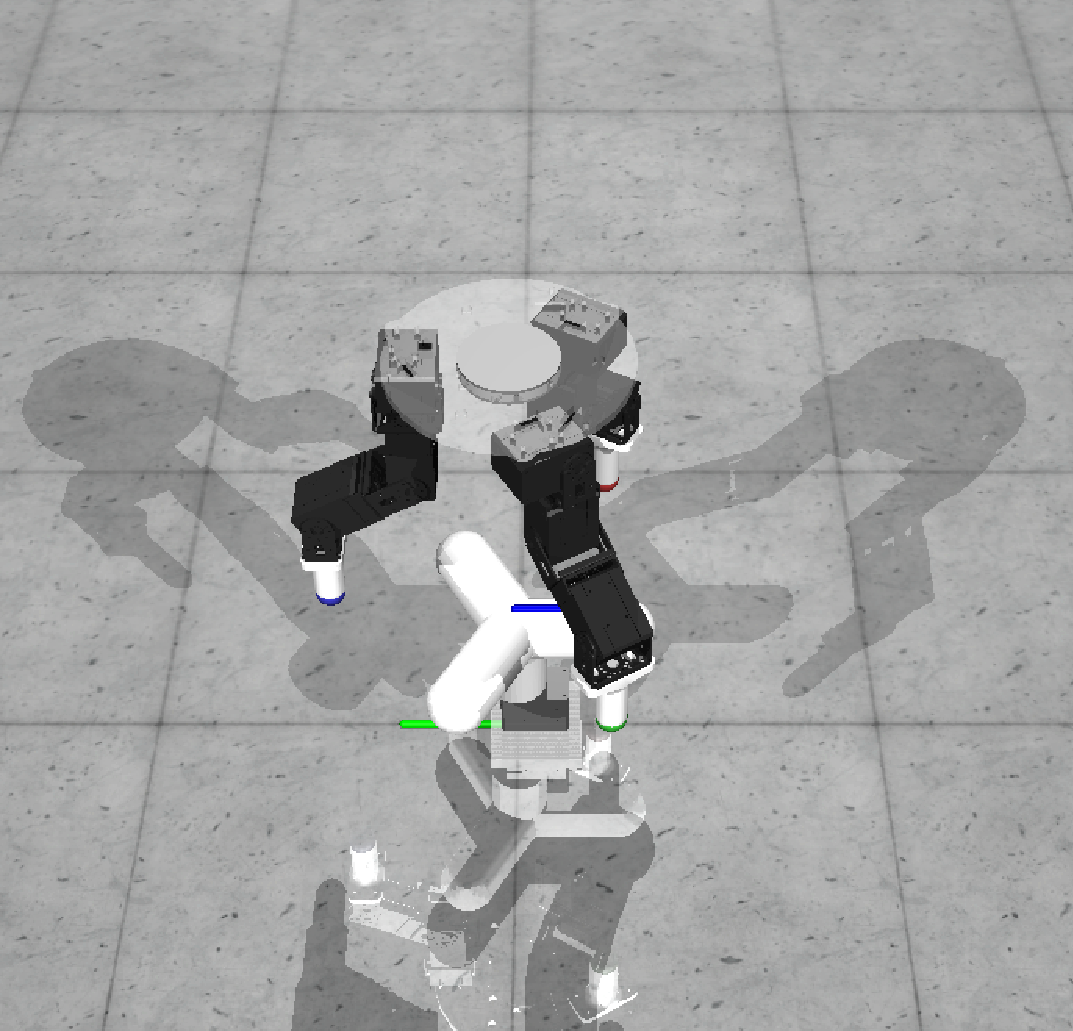
\includegraphics[height=10cm]
       {asset/img/dclaw_mujoco.pdf}
  \caption{物理エンジンMuJoCo上でのD'Claw.}
  \label{dclaw_mujoco}
\end{figure}



\subsubsection{実機の設定}
シミュレーター上で獲得した行動の低次元表現を用いて実機でのTurnタスクを学習する.図\ref{dclaw_hardware}に実機の写真を示す.実機は9つの関節を持ち,各関節とバルブの固定部にはアクチュエータが存在する.アクチュエータとしてはDynamixel XM430-W210を利用する.アクチュエータはPD位置制御で動作し,Pゲインは800,Dゲインは8000に設定している.また,ロボットの指先やバルブは3Dプリンターで作成したものであり,指先や3本足バルブのCADデータはRobelの公式サイトhttps://sites.google.com/view/roboticsbenchmarksで公開されているものを用いた.箱型バルブなどはどのようにして印刷した?
%%% 引用:https://emanual.robotis.com/docs/en/dxl/x/xm430-w210/ webサイトを引用する際のbibtexの記載は?
\begin{figure}[hbtp]
  \centering
  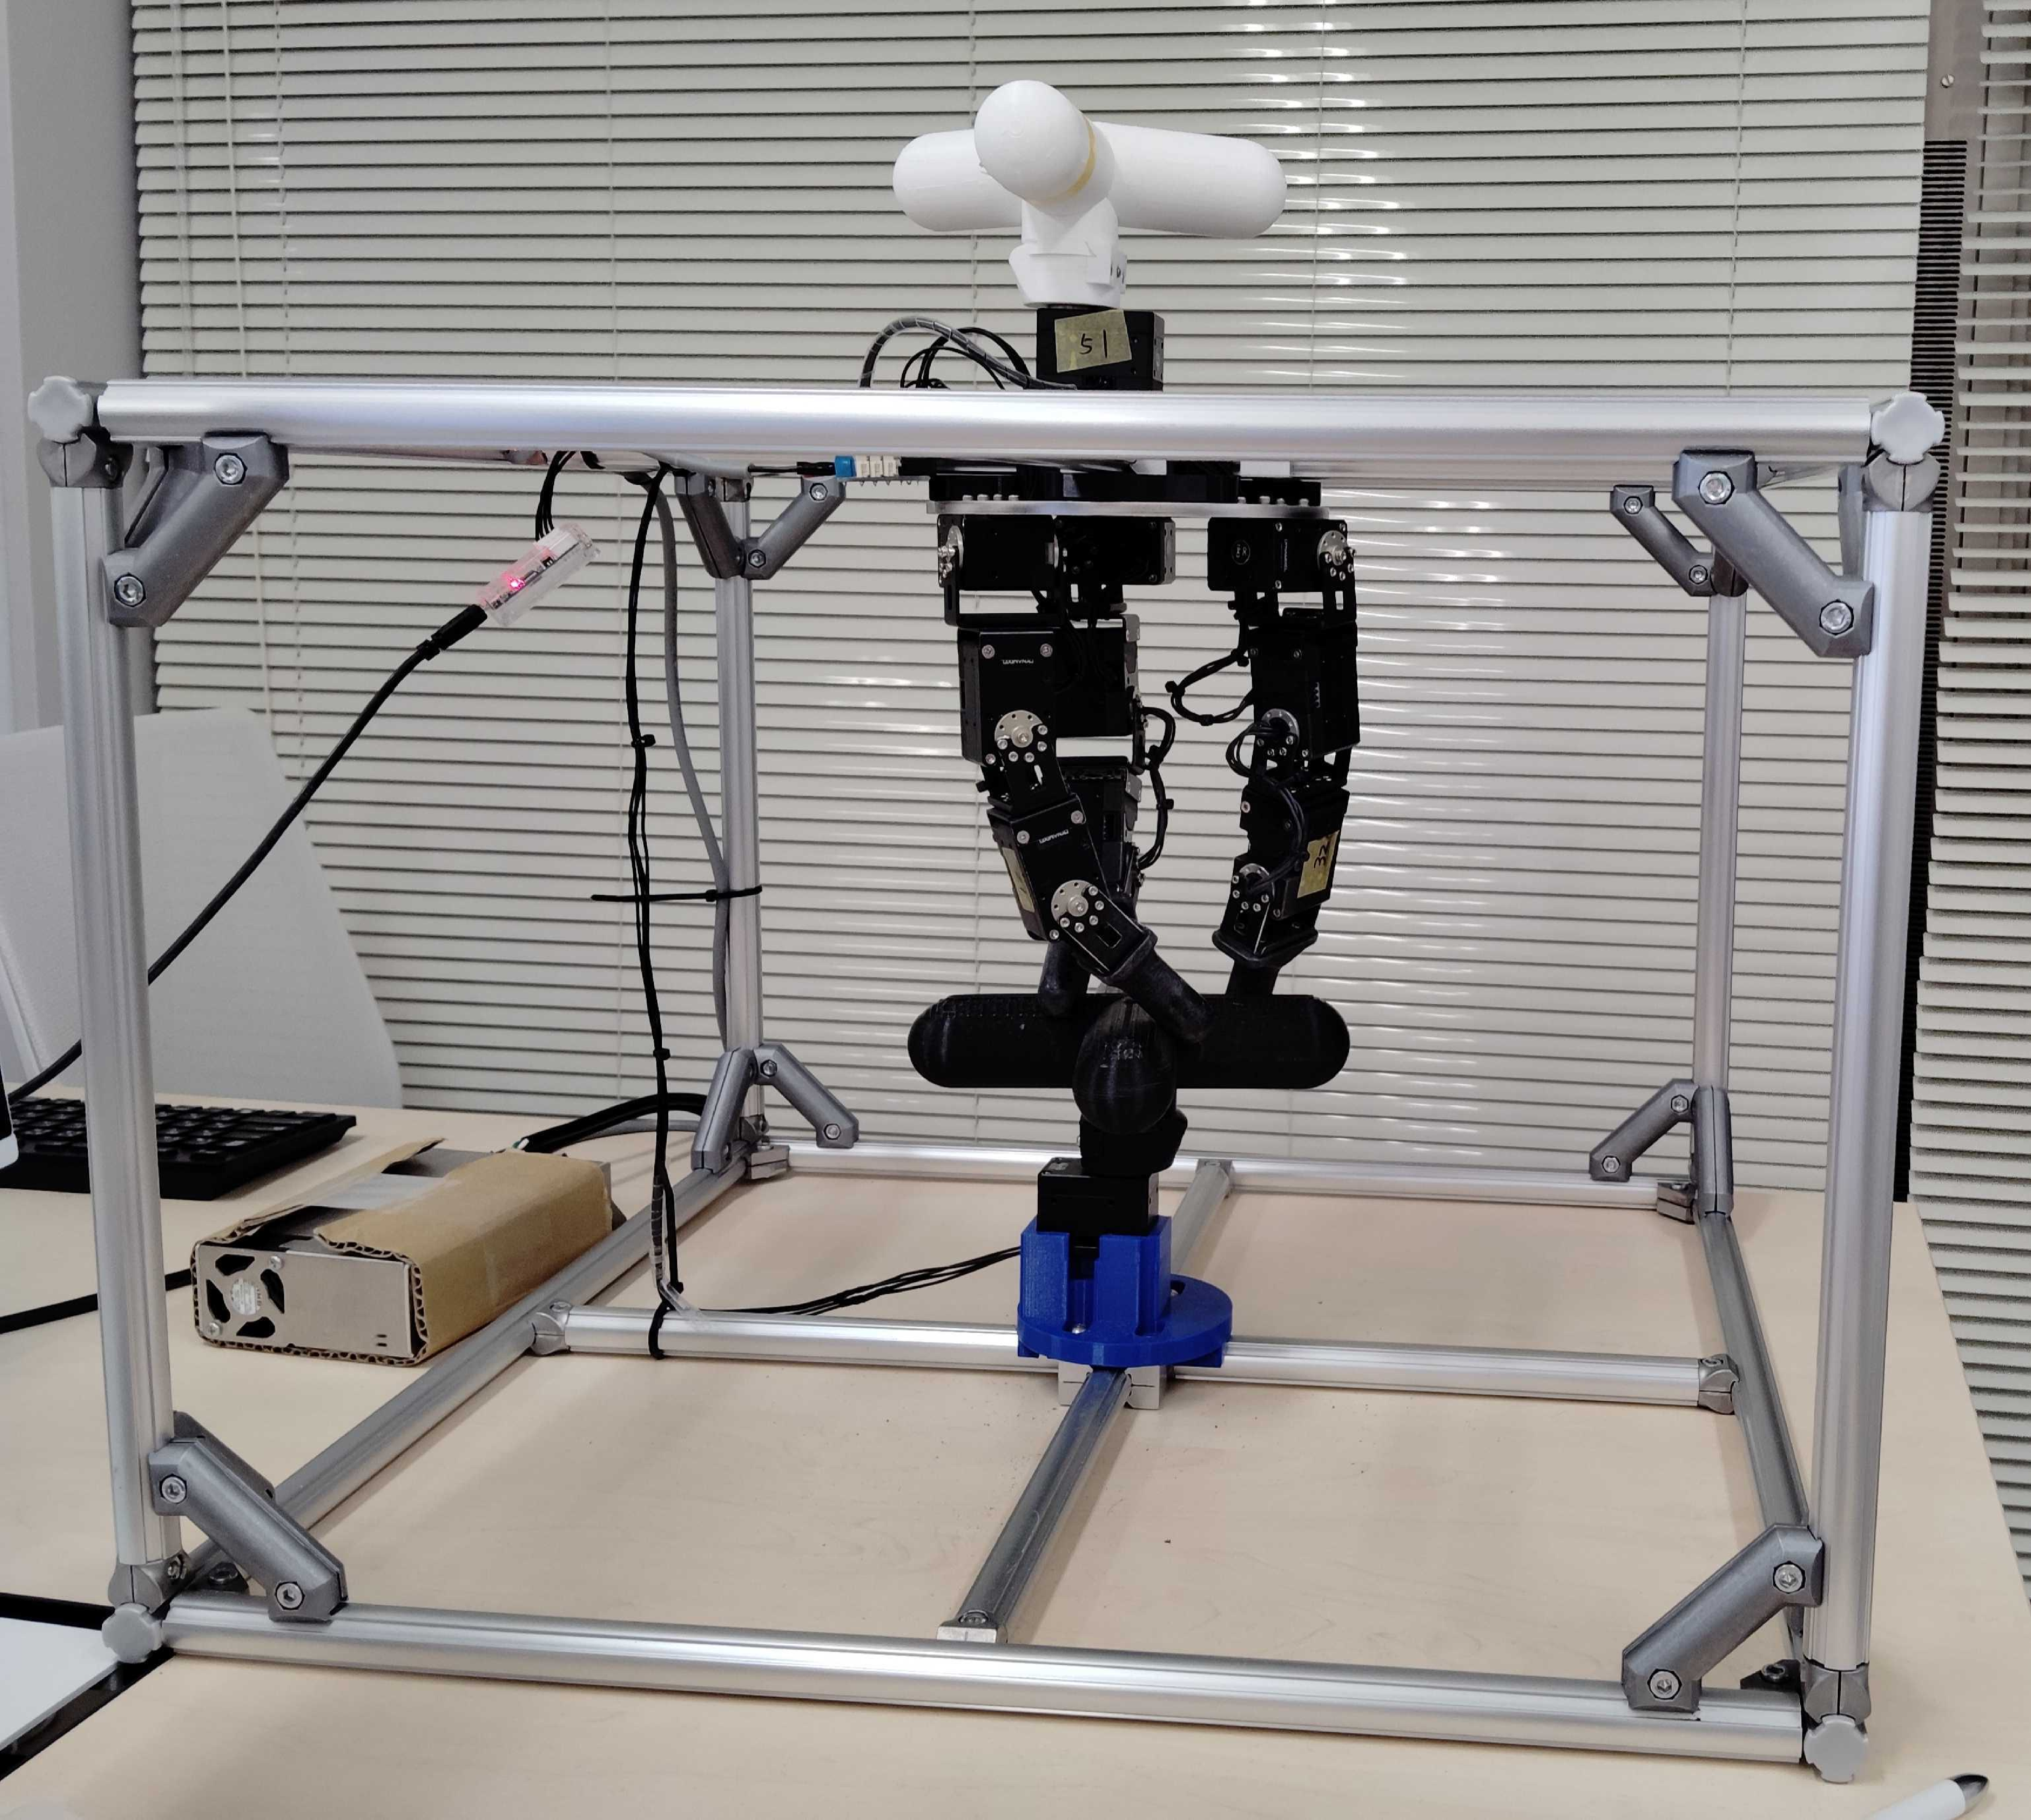
\includegraphics[height=10cm]
       {asset/img/dclaw_hardware.pdf}
  \caption{D'Clawの実機.}
  \label{dclaw_hardware}
\end{figure}

%%% バルブの画像を貼る.


\subsection{事前方策の収集}
低次元行動空間抽出のため,シミュレーション上でデータを収集する.データ収集には強化学習を利用し,アルゴリズムとしてはref{}で説明したSAC法を用いる.SAC法で学習させたのち,各方策についてバルブ角度の誤差が0.1以下になったエピソードを100エピソード分収集する.これを100個の方策について繰り返し,合わせて10000エピソードを学習用データとして用いた.
% 更に書くべき事項:確率的方策を実行したのか初期値をランダムにずらしたのか.→確率的方策を実行.
%・低次元行動空間抽出のため,事前にシミュレーション上で方策を収集.\\
%・SACを用いて120の方策を学習->120個以上ある場合もあったので.
% 100個の方策で確率的方策を実行し,バルブ角度の誤差が0.1以内に収まった100エピソード分データを集めた.
% 突っ込まれうるポイント:データの収集に用いているSACはRLbaseのものだが,比較に用いているSACはRLbaseをSPiRLに移植したもので学習速度が異なる.

\subsection{低次元行動空間の抽出}
強化学習の探索で用いる低次元空間を抽出するため変分オートエンコーダを学習する.変分オートエンコーダの学習には前節で収集した事前方策を元に生成した軌道データを用いる.変分オートエンコーダの学習は100Epoch行い,各Epochでは,全系列の中から をサンプリングしミニバッチ学習を行う.また,その他の変分オートエンコーダのパラメータ設定を表ref{}に示す.このような条件設定の下,潜在空間の次元を1,3,6,9と変化させ学習した場合の再構成誤差は図ref{}のようになった.次節以降では本節で抽出した低次元空間を用いて強化学習する.

%%% ******************VAEのモデル構成を説明する**********************

%前の項で説明したVAEを用いてデータを抽出.
%データのサンプリング方法.
%バッチサイズや学習率,エポック数などハイパーパラメータのセッティング.
%学習曲線を表示する.

\subsection{実験1:同一形状のバルブの学習(シミュレーション)}
・まず,抽出した低次元行動空間の性能を評価.\\
・データの存在するものと同一形状のバルブについて学習.\\
・SACのみ・ファインチューニングと比較.\\
・Ablation Studyとして,潜在変数の次元を変えて比較.\\
必要な図表:3種類の条件を比較した図・Ablation studyの図.\\
\begin{figure}[H]
  \centering
  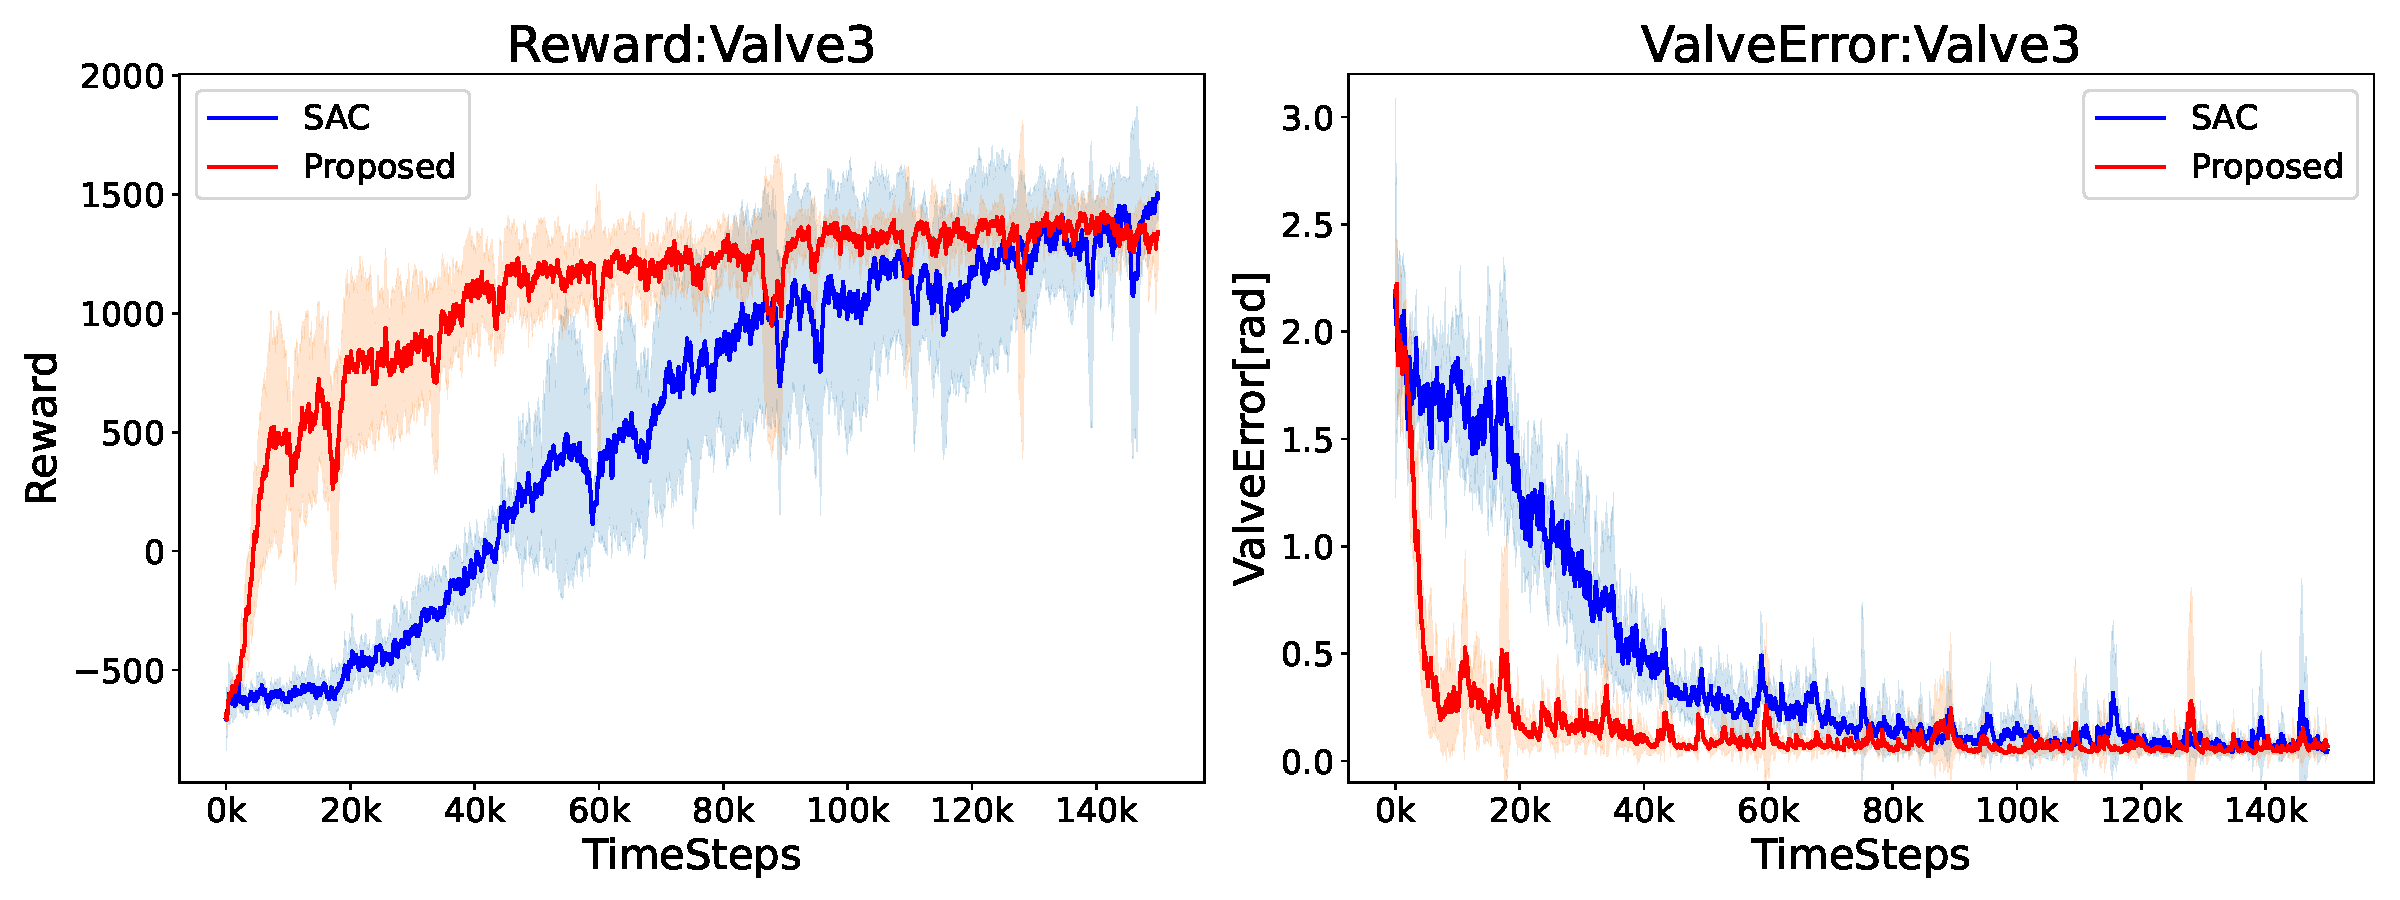
\includegraphics[width=16cm]
       {asset/img/SimTurn180Valve3.pdf}
  \caption{4種類のバルブにおける報酬とバルブ誤差の推移.}
  \label{dclaw_mujoco}
\end{figure}

\begin{figure}[H]
  \centering
  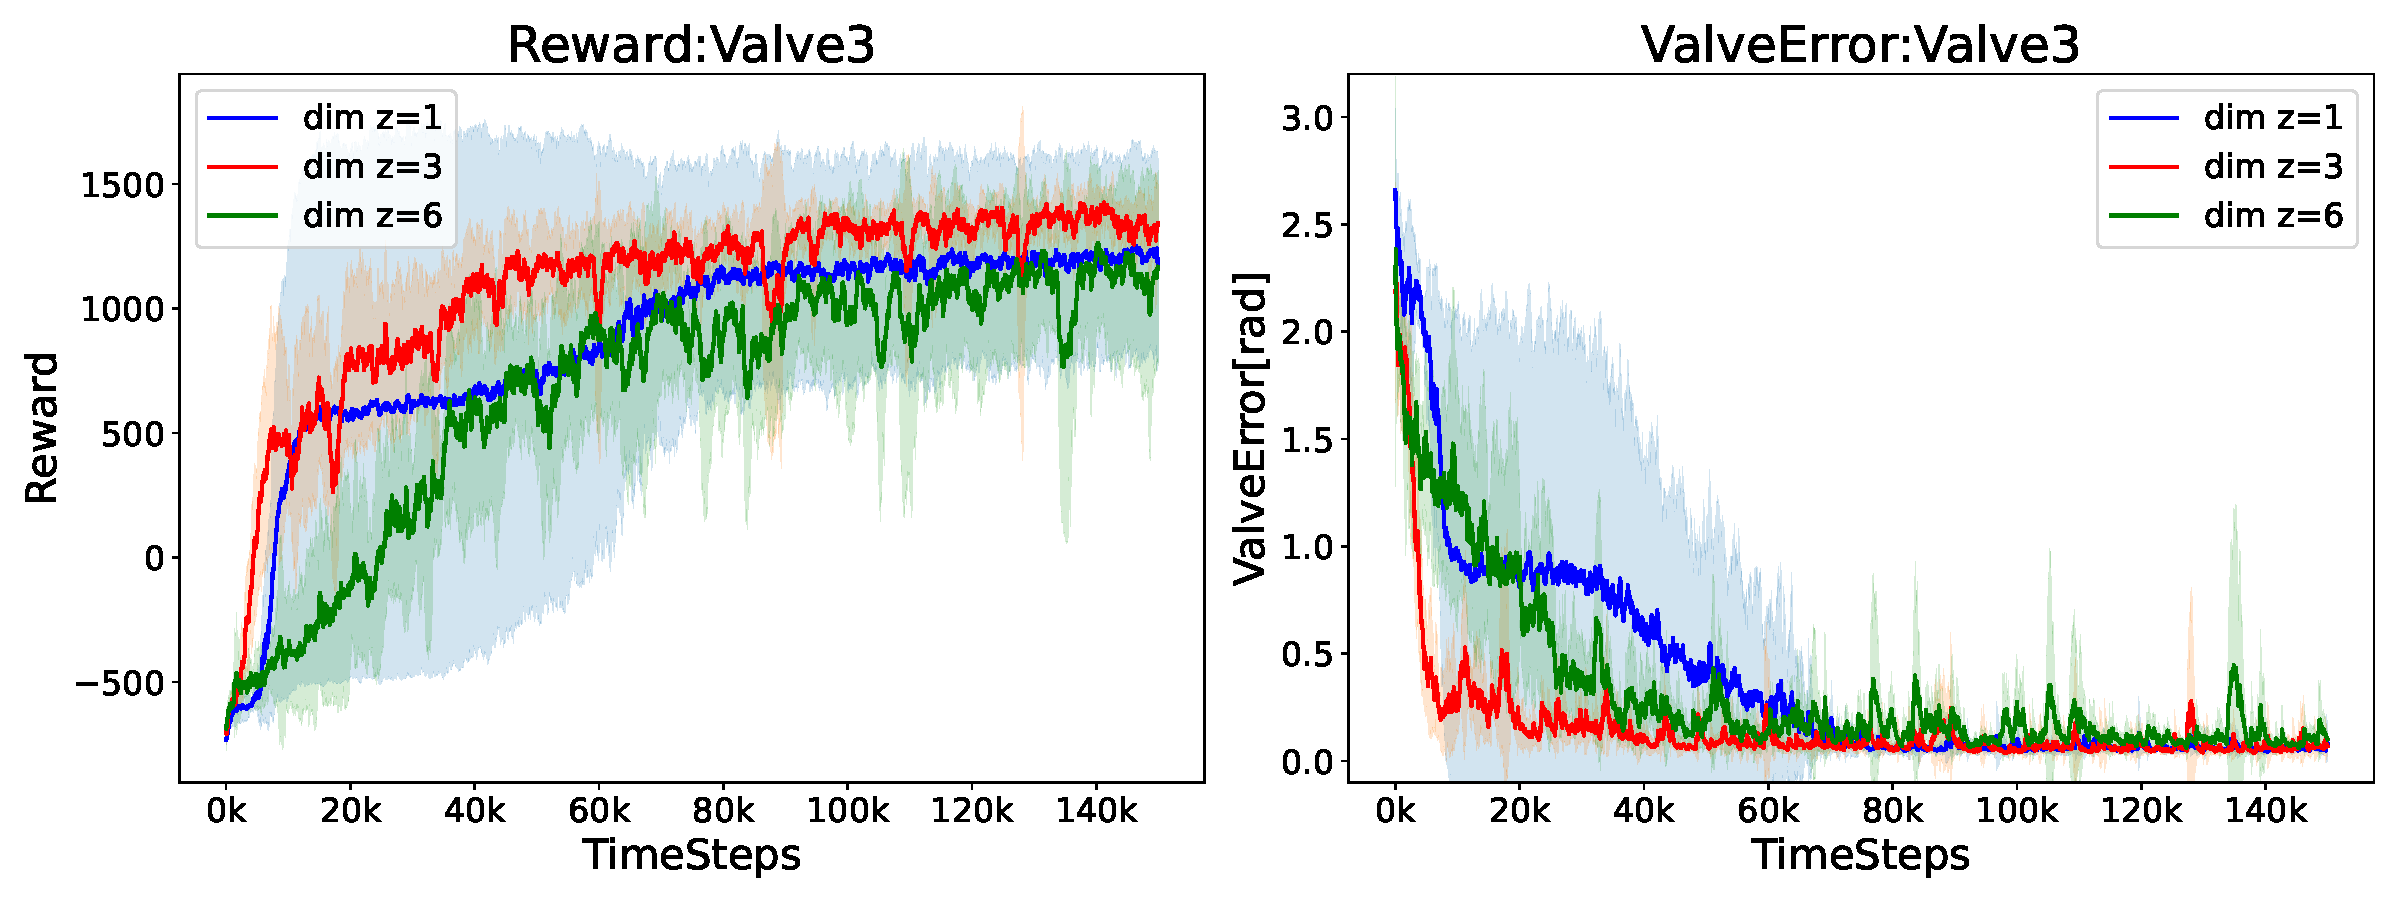
\includegraphics[width=16cm]
       {asset/img/SimValve3LatentDim.pdf}
  \caption{4種類のバルブにおける報酬とバルブ誤差の推移.}
  \label{dclaw_mujoco}
\end{figure}

\subsection{実験2:異なる形状のバルブへの転移(シミュレーション)}
・データの存在するものと異なる形状のバルブについて学習.\\
・まず,3本足バルブの方策をそのまま持っていくとどうなるかをまず.\\
・4種類のバルブについてSACのみ・ファインチューニングと比較.\\

\begin{figure}[H]
  \centering
  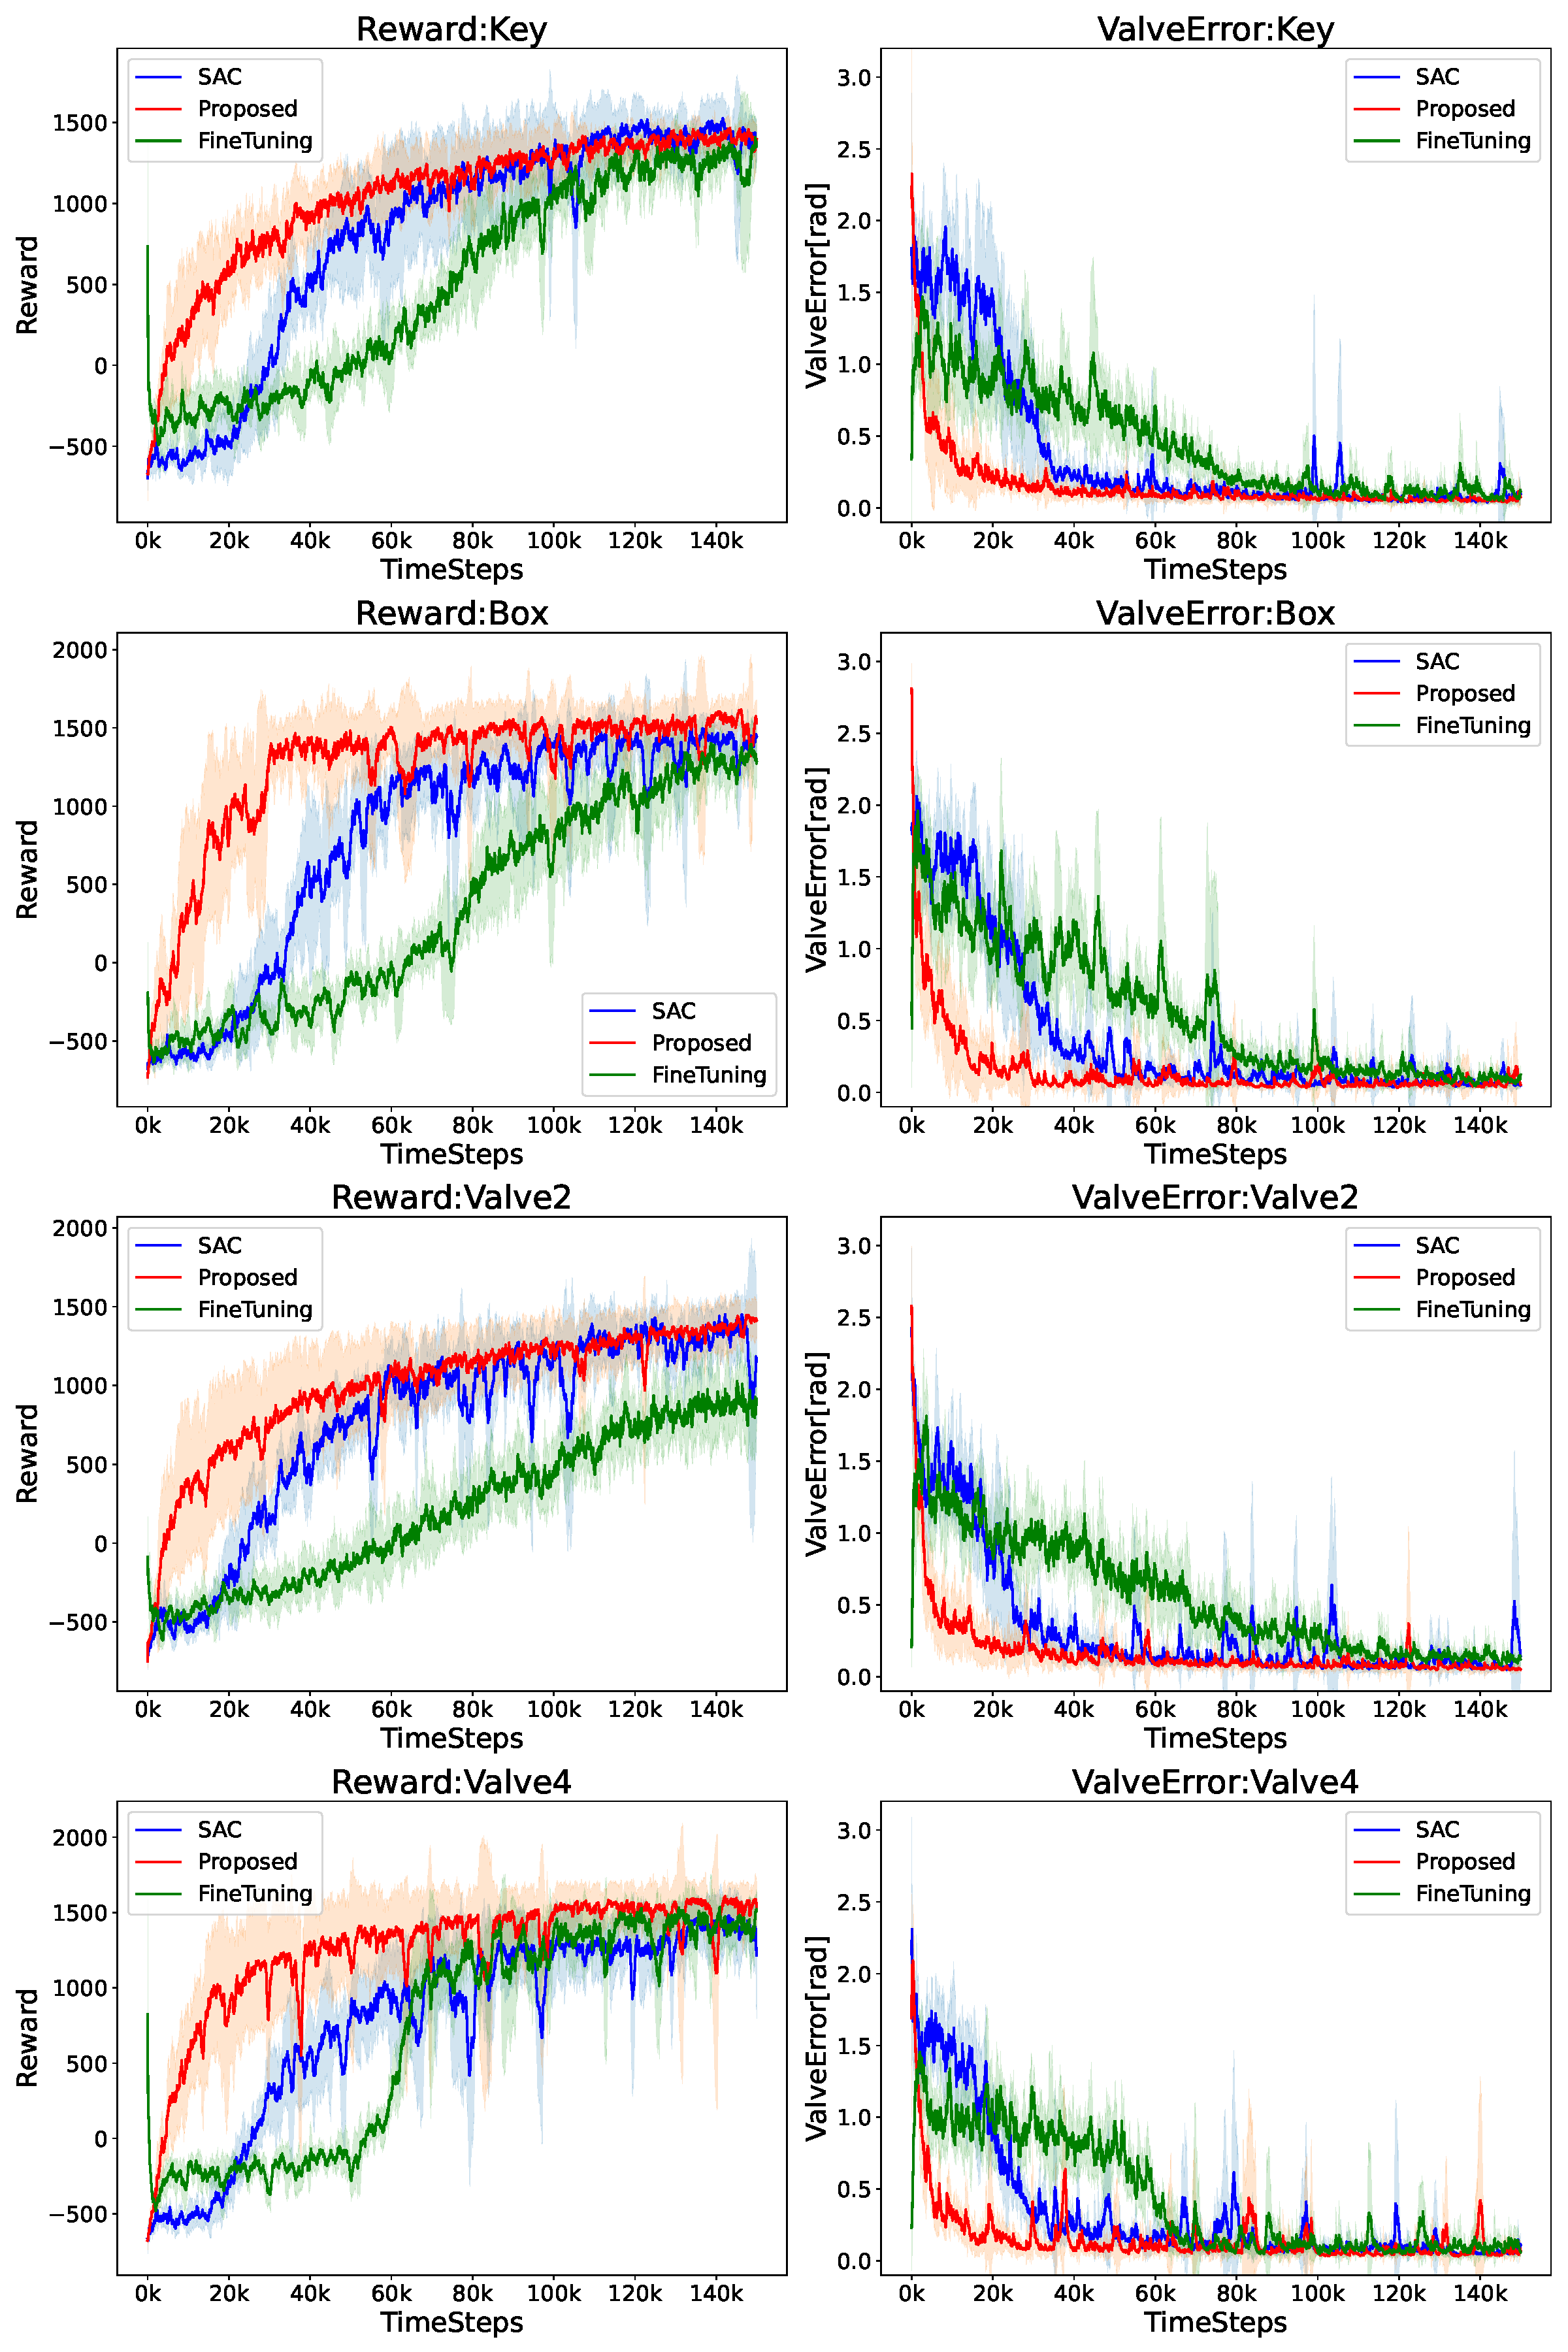
\includegraphics[width=16cm]
       {asset/img/SimTurn180Other.pdf}
  \caption{4種類のバルブにおける報酬とバルブ誤差の推移.}
  \label{dclaw_mujoco}
\end{figure}


\begin{figure}[H]
  \centering
  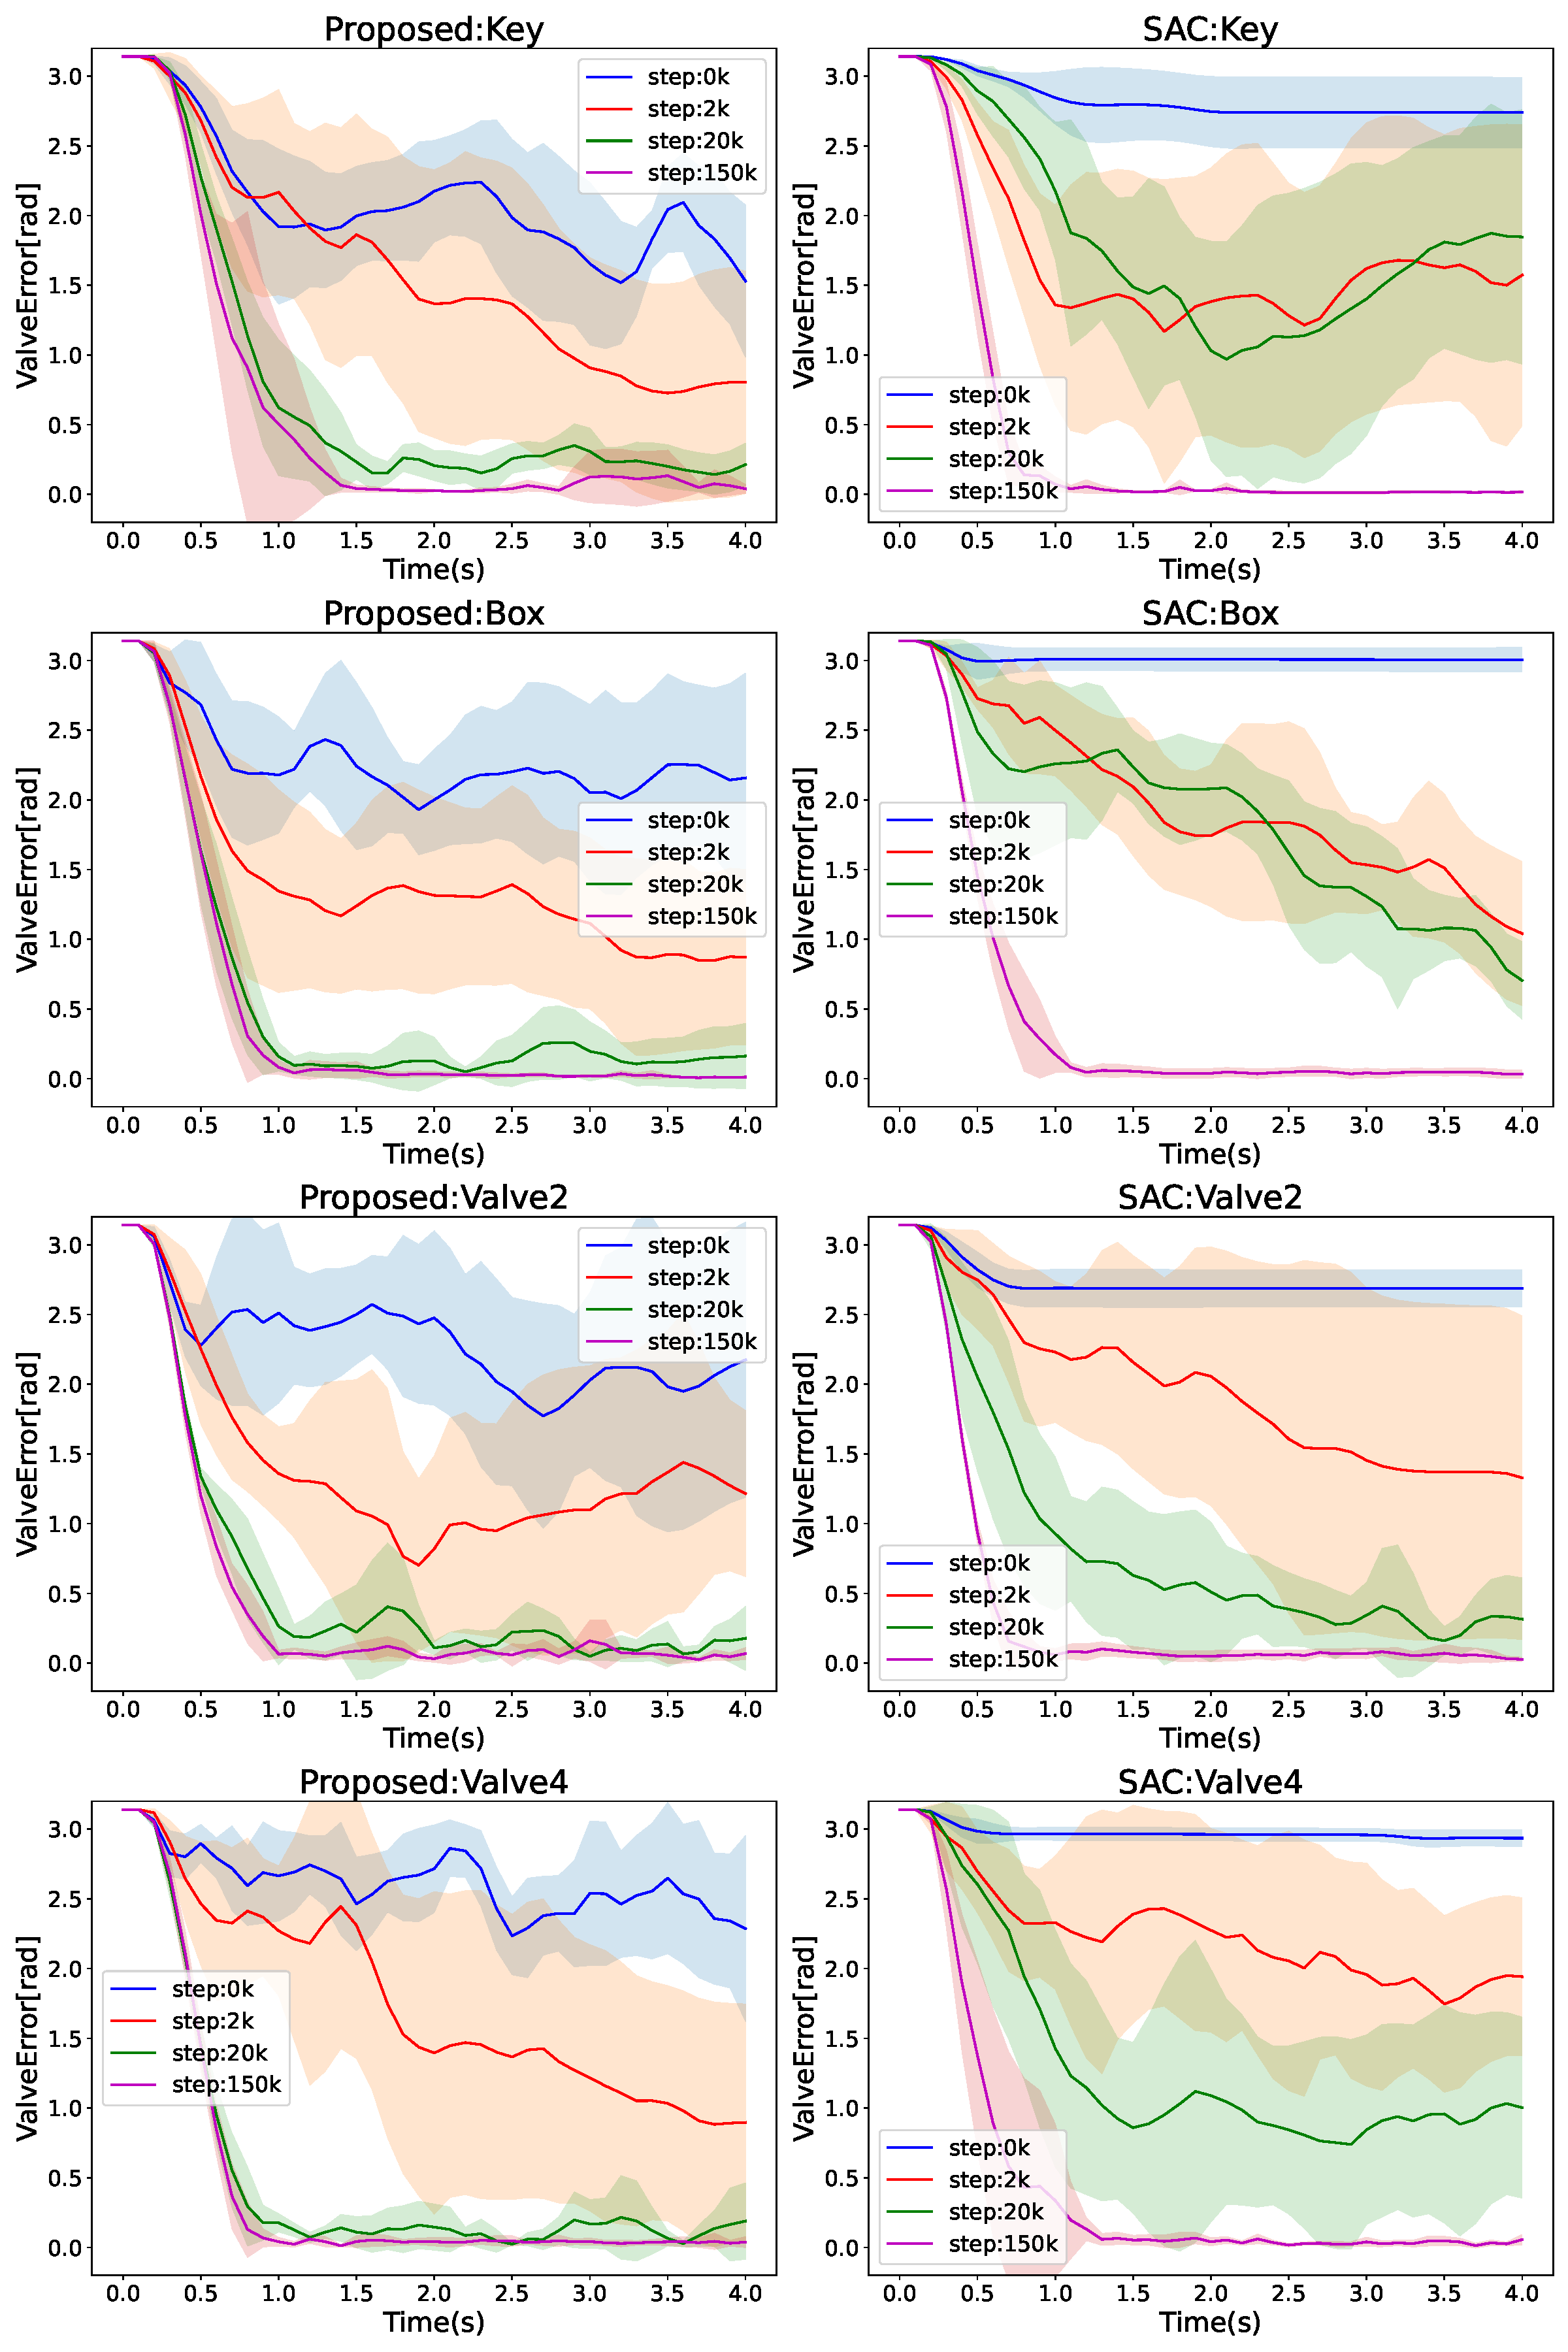
\includegraphics[width=16cm]
       {asset/img/ValveTrajectory_SimTurn180Other.pdf}
  \caption{事前方策と異なるバルブにおける学習中獲得した方策のバルブ角度誤差の軌道.}
  \label{dclaw_mujoco}
\end{figure}
・Ablation Studyとして,潜在変数の次元を変えて比較.\\
必要な図表:3本足の方策を4種類のバルブにそのまま持っていったときのバルブの誤差の表・4種類のバルブについて3種類の条件を比較した図・Ablation studyの図.\\

\subsection{実験3:同一形状のバルブの学習(実機)}
・提案したフレームワークをSimlation to realに利用できることを示す.
・まず,3本足バルブについてシミュレータで学習した方策をそのまま持っていくとどうなるかをまず.\\
・SACのみと比較.\\
・報酬の学習曲線・バルブ誤差の曲線を表示.

\begin{figure}[H]
  \centering
  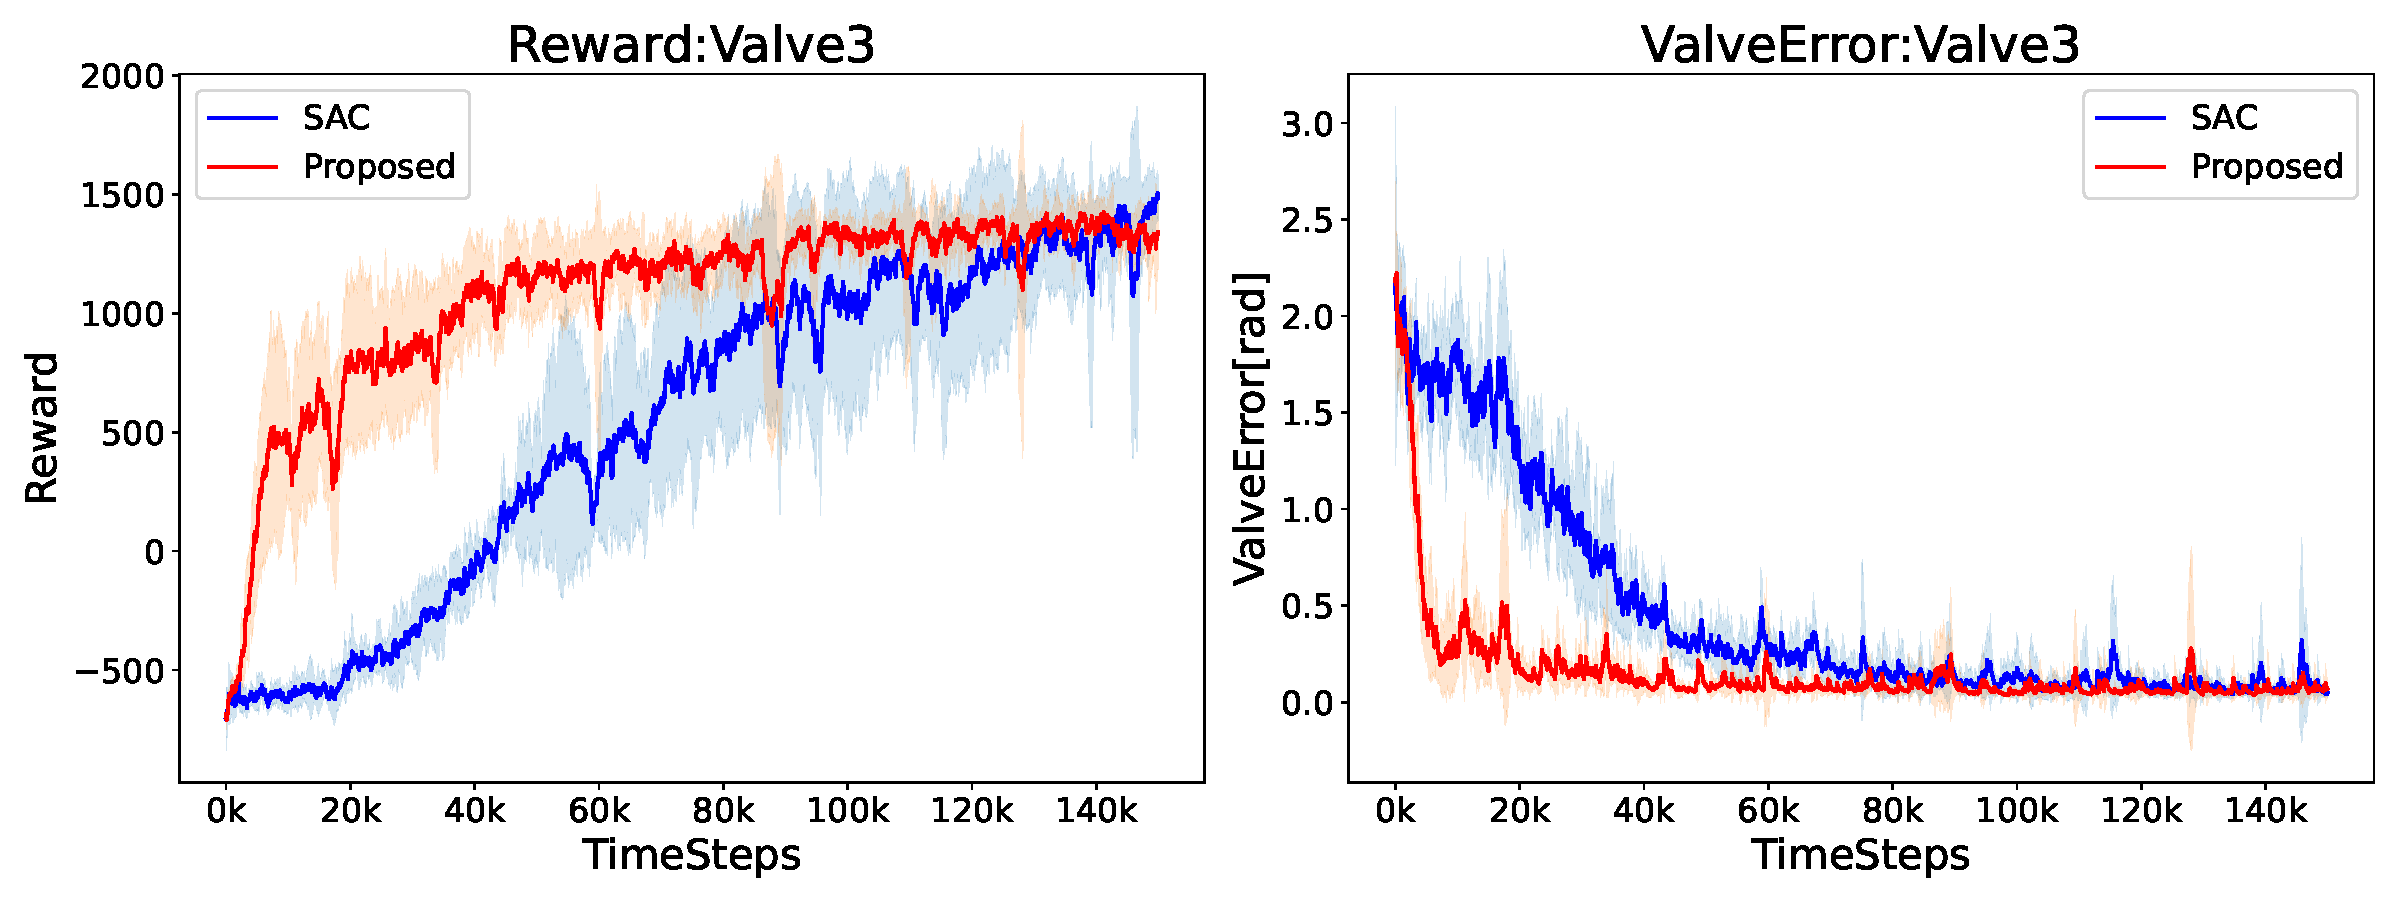
\includegraphics[width=16cm]
       {asset/img/HardwareTurn180.pdf}
  \caption{4種類のバルブにおける報酬とバルブ誤差の推移.}
  \label{dclaw_mujoco}
\end{figure}

\subsection{実験4:異なる形状のバルブへの転移(実機)}
・まず,3本足バルブについてシミュレータで学習した方策をそのまま持っていくとどうなるかをまず.\\
・4種類のバルブについてSACのみと比較.\\
必要な図表:
・3本足の方策を4種類のバルブにそのまま持っていったときのバルブの誤差の起動と比較
・4種類のバルブについて2種類の条件を比較した図.\\
実機ならではの図がほしい.


\clearpage
\section{議論}\label{sec-discussion}

\clearpage
\section{結論}\label{sec-conclusion}



%%% 謝辞 %%%%%%%%%%%%%%%%%%%%%%%%%%%%%%%%%%%%%%%%%%%%%%%%%%%%%%%%%%%%%%%%%%%%%%%%
\acknowledgment
に深く感謝する.

%%% 参考文献 %%%%%%%%%%%%%%%%%%%%%%%%%%%%%%%%%%%%%%%%%%%%%%%%%%%%%%%%%%%%%%%%%%%%
\addcontentsline{toc}{section}{\refname} % 目次に参考文献を追加する.
                                         % chapter使用時は削除すること.
\bibliographystyle{junsrt} % jplain.bstの読み込み.
\bibliography{thesis}

%%% BibTeX 等を用いる場合は,上の thebibliography 環境を消してここに該当コードを
%%% 挿入すること.
%% \bibliographystyle{...}
%% \bibliography{...}

%%% 付録 %%%%%%%%%%%%%%%%%%%%%%%%%%%%%%%%%%%%%%%%%%%%%%%%%%%%%%%%%%%%%%%%%%%%%%%%
%%% 付録は不要ならば削除してよい.
\appendix


%%% 本文ここまで %%%%%%%%%%%%%%%%%%%%%%%%%%%%%%%%%%%%%%%%%%%%%%%%%%%%%%%%%%%%%%%%
\fi
\ifoutputcover
\cleardoublepage
%%% 表紙,背表紙,提出用摘要 %%%%%%%%%%%%%%%%%%%%%%%%%%%%%%%%%%%%%%%%%%%%%%%%%%%%
\makecover                      % 表紙
\makespine[\numberofspines]     % 背表紙
\fi
\ifoutputabstractforsubmission
\makeabstractforsubmission      % 提出用摘要
\fi
\end{document}
